\documentclass[tikz,border=6pt]{standalone}
\usepackage{amsmath}
\usetikzlibrary{arrows.meta,calc,patterns,positioning}
\begin{document}

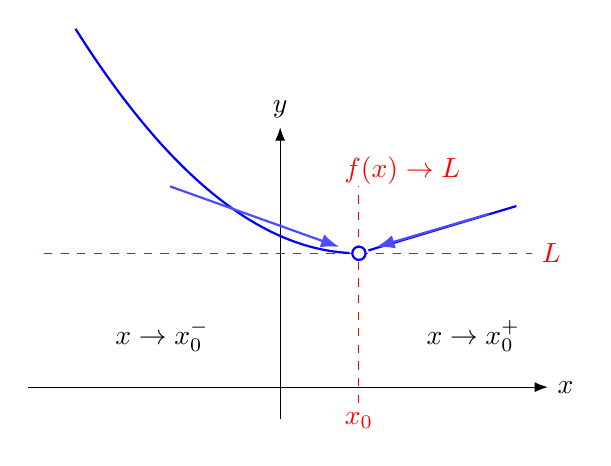
\begin{tikzpicture}[>=Latex,scale=1]
  \draw[->] (-3.2,0) -- (3.4,0) node[right] {$x$};
  \draw[->] (0,-0.4) -- (0,3.3) node[above] {$y$};
  \draw[dashed,red] (1,-0.2) node[below] {$x_0$} -- (1,2.55);
  \draw[dashed,red] (-3,1.7) -- (3.2,1.7) node[right] {$L$};
  \draw[domain=-2.6:0.88,smooth,variable=\x,blue,thick] plot ({\x},{1.7+0.22*(\x-1)*(\x-1)});
  \draw[domain=1.12:3.0,smooth,variable=\x,blue,thick] plot ({\x},{1.7+0.30*(\x-1)});
  \draw[->,blue!70,thick] (-1.4,2.55) -- (0.75,1.78);
  \draw[->,blue!70,thick] (2.65,2.20) -- (1.22,1.78);
  \fill[white,draw=blue,thick] (1,1.7) circle (2.4pt);
  \node[align=center] at (-1.5,0.65) {$x\to x_0^-$};
  \node[align=center] at (2.45,0.65) {$x\to x_0^+$};
  \node[red] at (1.55,2.75) {$f(x)\to L$};
\end{tikzpicture}

\end{document}
